\PassOptionsToPackage{unicode=true}{hyperref} % options for packages loaded elsewhere
\PassOptionsToPackage{hyphens}{url}
%
\documentclass[]{article}
\usepackage{lmodern}
\usepackage{amssymb,amsmath}
\usepackage{ifxetex,ifluatex}
\usepackage{fixltx2e} % provides \textsubscript
\ifnum 0\ifxetex 1\fi\ifluatex 1\fi=0 % if pdftex
  \usepackage[T1]{fontenc}
  \usepackage[utf8]{inputenc}
  \usepackage{textcomp} % provides euro and other symbols
\else % if luatex or xelatex
  \usepackage{unicode-math}
  \defaultfontfeatures{Ligatures=TeX,Scale=MatchLowercase}
\fi
% use upquote if available, for straight quotes in verbatim environments
\IfFileExists{upquote.sty}{\usepackage{upquote}}{}
% use microtype if available
\IfFileExists{microtype.sty}{%
\usepackage[]{microtype}
\UseMicrotypeSet[protrusion]{basicmath} % disable protrusion for tt fonts
}{}
\IfFileExists{parskip.sty}{%
\usepackage{parskip}
}{% else
\setlength{\parindent}{0pt}
\setlength{\parskip}{6pt plus 2pt minus 1pt}
}
\usepackage{hyperref}
\hypersetup{
            pdfborder={0 0 0},
            breaklinks=true}
\urlstyle{same}  % don't use monospace font for urls
\usepackage{color}
\usepackage{fancyvrb}
\newcommand{\VerbBar}{|}
\newcommand{\VERB}{\Verb[commandchars=\\\{\}]}
\DefineVerbatimEnvironment{Highlighting}{Verbatim}{commandchars=\\\{\}}
% Add ',fontsize=\small' for more characters per line
\newenvironment{Shaded}{}{}
\newcommand{\AlertTok}[1]{\textcolor[rgb]{1.00,0.00,0.00}{\textbf{#1}}}
\newcommand{\AnnotationTok}[1]{\textcolor[rgb]{0.38,0.63,0.69}{\textbf{\textit{#1}}}}
\newcommand{\AttributeTok}[1]{\textcolor[rgb]{0.49,0.56,0.16}{#1}}
\newcommand{\BaseNTok}[1]{\textcolor[rgb]{0.25,0.63,0.44}{#1}}
\newcommand{\BuiltInTok}[1]{#1}
\newcommand{\CharTok}[1]{\textcolor[rgb]{0.25,0.44,0.63}{#1}}
\newcommand{\CommentTok}[1]{\textcolor[rgb]{0.38,0.63,0.69}{\textit{#1}}}
\newcommand{\CommentVarTok}[1]{\textcolor[rgb]{0.38,0.63,0.69}{\textbf{\textit{#1}}}}
\newcommand{\ConstantTok}[1]{\textcolor[rgb]{0.53,0.00,0.00}{#1}}
\newcommand{\ControlFlowTok}[1]{\textcolor[rgb]{0.00,0.44,0.13}{\textbf{#1}}}
\newcommand{\DataTypeTok}[1]{\textcolor[rgb]{0.56,0.13,0.00}{#1}}
\newcommand{\DecValTok}[1]{\textcolor[rgb]{0.25,0.63,0.44}{#1}}
\newcommand{\DocumentationTok}[1]{\textcolor[rgb]{0.73,0.13,0.13}{\textit{#1}}}
\newcommand{\ErrorTok}[1]{\textcolor[rgb]{1.00,0.00,0.00}{\textbf{#1}}}
\newcommand{\ExtensionTok}[1]{#1}
\newcommand{\FloatTok}[1]{\textcolor[rgb]{0.25,0.63,0.44}{#1}}
\newcommand{\FunctionTok}[1]{\textcolor[rgb]{0.02,0.16,0.49}{#1}}
\newcommand{\ImportTok}[1]{#1}
\newcommand{\InformationTok}[1]{\textcolor[rgb]{0.38,0.63,0.69}{\textbf{\textit{#1}}}}
\newcommand{\KeywordTok}[1]{\textcolor[rgb]{0.00,0.44,0.13}{\textbf{#1}}}
\newcommand{\NormalTok}[1]{#1}
\newcommand{\OperatorTok}[1]{\textcolor[rgb]{0.40,0.40,0.40}{#1}}
\newcommand{\OtherTok}[1]{\textcolor[rgb]{0.00,0.44,0.13}{#1}}
\newcommand{\PreprocessorTok}[1]{\textcolor[rgb]{0.74,0.48,0.00}{#1}}
\newcommand{\RegionMarkerTok}[1]{#1}
\newcommand{\SpecialCharTok}[1]{\textcolor[rgb]{0.25,0.44,0.63}{#1}}
\newcommand{\SpecialStringTok}[1]{\textcolor[rgb]{0.73,0.40,0.53}{#1}}
\newcommand{\StringTok}[1]{\textcolor[rgb]{0.25,0.44,0.63}{#1}}
\newcommand{\VariableTok}[1]{\textcolor[rgb]{0.10,0.09,0.49}{#1}}
\newcommand{\VerbatimStringTok}[1]{\textcolor[rgb]{0.25,0.44,0.63}{#1}}
\newcommand{\WarningTok}[1]{\textcolor[rgb]{0.38,0.63,0.69}{\textbf{\textit{#1}}}}
\usepackage{longtable,booktabs}
% Fix footnotes in tables (requires footnote package)
\IfFileExists{footnote.sty}{\usepackage{footnote}\makesavenoteenv{longtable}}{}
\usepackage{graphicx,grffile}
\makeatletter
\def\maxwidth{\ifdim\Gin@nat@width>\linewidth\linewidth\else\Gin@nat@width\fi}
\def\maxheight{\ifdim\Gin@nat@height>\textheight\textheight\else\Gin@nat@height\fi}
\makeatother
% Scale images if necessary, so that they will not overflow the page
% margins by default, and it is still possible to overwrite the defaults
% using explicit options in \includegraphics[width, height, ...]{}
\setkeys{Gin}{width=\maxwidth,height=\maxheight,keepaspectratio}
\setlength{\emergencystretch}{3em}  % prevent overfull lines
\providecommand{\tightlist}{%
  \setlength{\itemsep}{0pt}\setlength{\parskip}{0pt}}
\setcounter{secnumdepth}{0}
% Redefines (sub)paragraphs to behave more like sections
\ifx\paragraph\undefined\else
\let\oldparagraph\paragraph
\renewcommand{\paragraph}[1]{\oldparagraph{#1}\mbox{}}
\fi
\ifx\subparagraph\undefined\else
\let\oldsubparagraph\subparagraph
\renewcommand{\subparagraph}[1]{\oldsubparagraph{#1}\mbox{}}
\fi

% set default figure placement to htbp
\makeatletter
\def\fps@figure{htbp}
\makeatother


\date{}

\begin{document}

\hypertarget{header-n3}{%
\section{Abstract}\label{header-n3}}

\hypertarget{header-n5}{%
\section{1. Introduction}\label{header-n5}}

\hypertarget{header-n6}{%
\section{2. Symbolic Execution}\label{header-n6}}

\hypertarget{header-n7}{%
\subsection{2.1 Introduction to Symbolic Execution}\label{header-n7}}

Symbolic execution is a technique for testing program correctness
initially proposed in the 1970s \footnote{King, J. C. (1976). Symbolic
  execution and program testing. \emph{Communications of the ACM},
  \emph{19}(7), 385-394.}\footnote{Boyer, R. S., Elspas, B., \& Levitt,
  K. N. (1975). SELECT---a formal system for testing and debugging
  programs by symbolic execution. \emph{ACM SigPlan Notices},
  \emph{10}(6), 234-245.}. Classically, it's the process of executing a
program by representing its variables as arbitrary symbols rather than
concrete values. Execution of the program occurs using these symbolic
inputs by extending the basic operators and semantics of the program's
language to use symbols and produce symbolic formulas rather than
concrete values. In doing so, each symbolic execution tests many actual
instances of execution. \texttt{If} statements and language features
that cause execution to diverge are represented as a path condition, a
conjunction of conditions on symbols that must be satisfied. Evaluating
the constraint allows you to identify whether a path is feasible and if
so, the satisfied constraint provides the set of concrete inputs that
the path could be run under \footnote{Bierman, G., Abadi, M., \&
  Torgersen, M. (2014, July). Understanding typescript. In
  \emph{European Conference on Object-Oriented Programming} (pp.
  257-281). Springer, Berlin, Heidelberg.}. At the end of execution the
path condition, the conjunction of branch conditions taken to the
current point of execution, provides a unique representation of a path
tested through the program and when solved using a constraint solver
produces a set of inputs that when run take the same path through the
program as the symbolic execution \footnote{Godefroid, P., Levin, M. Y.,
  \& Molnar, D. A. (2008, February). Automated whitebox fuzz testing. In
  \emph{NDSS} (Vol. 8, pp. 151-166).}, \footnote{Godefroid, P.,
  Klarlund, N., \& Sen, K. (2005, June). DART: directed automated random
  testing. In \emph{ACM Sigplan Notices} (Vol. 40, No. 6, pp. 213-223).
  ACM.}. By exploring a program's paths exhaustively (or as thoroughly
as possible within either a time or path count constraint) combining
symbolic execution with techniques to compare symbolic output with
expected values it's possible to test program correctness \footnote{King,
  J. C. (1976). Symbolic execution and program testing.
  \emph{Communications of the ACM}, \emph{19}(7), 385-394.}.

\emph{Figure 1: Absolute Sum Function}

\begin{Shaded}
\begin{Highlighting}[]
\DecValTok{1} \KeywordTok{function} \AttributeTok{abs_sum}\NormalTok{ (x}\OperatorTok{,}\NormalTok{ y)}\OperatorTok{\{}
\DecValTok{2}  \ControlFlowTok{if}\NormalTok{ (x }\OperatorTok{<} \DecValTok{0}\NormalTok{)}
\DecValTok{3}\NormalTok{    x }\OperatorTok{=}\NormalTok{ x }\OperatorTok{*} \DecValTok{-1}
\DecValTok{4}  \ControlFlowTok{if}\NormalTok{ (y }\OperatorTok{<} \DecValTok{0}\NormalTok{)}
\DecValTok{5}\NormalTok{    y }\OperatorTok{=}\NormalTok{ y }\OperatorTok{*} \DecValTok{-1}
\DecValTok{6}  \ControlFlowTok{return}\NormalTok{ x }\OperatorTok{+}\NormalTok{ y}
\DecValTok{7} \OperatorTok{\}}
\end{Highlighting}
\end{Shaded}

For example, consider the program above (fig. 1) which returns the sum
of the absolute values of two values. There are four possible paths that
can be taken through the program. The first is where neither if branches
are entered, the second is where the value of \texttt{x} is less than
zero, the third is where the value of \texttt{y} is less than zero, and
the fourth is where both \texttt{x} and \texttt{y} is less than zero.
The process for symbolically executing this program classically is as
follows. The function is executed with two symbolic values \(x'\) and
\(y'\) and a path condition \(pc\), "the accumulator of properties which
inputs must satisfy ... to follow ... a particular path" \footnote{King,
  J. C. (1976). Symbolic execution and program testing.
  \emph{Communications of the ACM}, \emph{19}(7), 385-394.}, is
initialised to \(true\). When a branching statement (line 2 or 4) is
reached the constraint solver is queried to see if the branch condition
is feasible given the current path condition. If condition is
satisfiable then execution forks to explore the new path and \(pc\)
becomes \(pc \land bc\) , where \(bc\) is the branch condition. This
process repeats until the program terminates and every path is explored.
The table below shows the path condition, symbolic results, and the
constraint solver queries and results for the execution.

\begin{longtable}[]{@{}llll@{}}
\toprule
\(pc\) & Result & Constraint Solver Queries & Query
Result\tabularnewline
\midrule
\endhead
\(x >= \land y >= 0\) & \(x+y\) & \(x >=0 \land y < 0 \) &
SAT\tabularnewline
\(x >= \land y < 0\) & \(x - y\) & \(x <0 \) & SAT\tabularnewline
\(x < \land y >= 0\) & \(-x+y\) & \(x<0 \land y < 0 \) &
SAT\tabularnewline
\(x < \land y < 0\) & \(-x-y\) & &\tabularnewline
\bottomrule
\end{longtable}

Historically, this technique has been impractical due to the limitations
on computing resources and the capabilities of automated theorem
provers\footnote{King, J. C. (1976). Symbolic execution and program
  testing. \emph{Communications of the ACM}, \emph{19}(7), 385-394.}
however in the 2000s there was a a number of advancements in the
technique by DART\footnote{Godefroid, P., Klarlund, N., \& Sen, K.
  (2005, June). DART: directed automated random testing. In \emph{ACM
  Sigplan Notices} (Vol. 40, No. 6, pp. 213-223). ACM.} and EXE
\footnote{Cadar, C., Ganesh, V., Pawlowski, P. M., Dill, D. L., \&
  Engler, D. R. (2008). EXE: automatically generating inputs of death.
  \emph{ACM Transactions on Information and System Security (TISSEC)},
  \emph{12}(2), 10.} made feasible due to the improvements in computer
hardware and the improvement of solvers\footnote{De Moura, L., \&
  Bjørner, N. (2011). Satisfiability modulo theories: introduction and
  applications. \emph{Communications of the ACM}, \emph{54}(9), 69-77.}
.

In these modern implementations, the program is run both concretely and
symbolically in so called concolic execution. In concolic execution, the
program is instrumented to run concretely whilst the program state is
shadowed by symbolic variables allowing the concrete execution to
'drive' the symbolic execution. Unlike pure symbolic execution, concolic
execution requires its initial input to be concrete, this input can be
random or crafted to fit the target program\footnote{Godefroid, P.,
  Kiezun, A., \& Levin, M. Y. (2008, June). Grammar-based whitebox
  fuzzing. In \emph{ACM Sigplan Notices} (Vol. 43, No. 6, pp. 206-215).
  ACM.}, \footnote{Cadar, C., \& Sen, K. (2013). Symbolic execution for
  software testing: three decades later. \emph{Communications of the
  ACM}, \emph{56}(2), 82-90.}. As concolic execution concretely executes
programs, rather than just modelling the semantics of the language you
can be sure that any bugs found are actual bugs. Additionally, when a
constraint cannot be solved concolic execution allows concrete values to
be substituted for unsolvable elements of constraints \footnote{Sen, K.
  (2007, November). Concolic testing. In \emph{Proceedings of the
  twenty-second IEEE/ACM international conference on Automated software
  engineering} (pp. 571-572). ACM.}, \footnote{Sen, K., Marinov, D., \&
  Agha, G. (2005, September). CUTE: a concolic unit testing engine for
  C. In \emph{ACM SIGSOFT Software Engineering Notes} (Vol. 30, No. 5,
  pp. 263-272). ACM.}.

Consider the following example of concolic execution testing the program
described in figure 1. Inputs for \texttt{x} and \texttt{y} are randomly
generated, for instance \texttt{x=217} and \texttt{y=931}. These then
guide the execution to not visit any branches, producing the \(pc\) of
\(x >= 0 \land y >=0\), this path condition can then be negated to
produce further paths. Using the DART\footnote{Godefroid, P., Klarlund,
  N., \& Sen, K. (2005, June). DART: directed automated random testing.
  In \emph{ACM Sigplan Notices} (Vol. 40, No. 6, pp. 213-223). ACM.}
style directed symbolic execution the following paths are generated.

\begin{longtable}[]{@{}lllll@{}}
\toprule
Input (x, y) & \(pc\) & Result & Constraint Solver Queries & Query
Result\tabularnewline
\midrule
\endhead
0, 0 & \(x >= \land y >= 0\) & \(x+y\) & \(x >=0 \land y < 0 \) &
SAT\tabularnewline
0, -3 & \(x >= \land y < 0\) & \(x - y\) & \(x <0 \) &
SAT\tabularnewline
-2, 1 & \(x < \land y >= 0\) & \(-x+y\) & \(x<0 \land y < 0 \) &
SAT\tabularnewline
-2, -7 & \(x < \land y < 0\) & \(-x-y\) & &\tabularnewline
\bottomrule
\end{longtable}

\hypertarget{header-n78}{%
\subsubsection{2.2 Finding and Choosing Paths}\label{header-n78}}

Although in theory symbolic execution will exhaustively search through
all feasible paths, as the length of the program under test increases
the number of paths in the program increases roughly exponentially
\footnote{Cadar, C., \& Sen, K. (2013). Symbolic execution for software
  testing: three decades later. \emph{Communications of the ACM},
  \emph{56}(2), 82-90.}. As these symbolic execution tools are bounded
by real world time constraint, paths must be chosen carefully in order
to prioritise exploring 'interesting' cases in the time available.

In EXE, and other more traditional methods, paths are found by building
a control flow graph and then exploring the graph using a form of
breadth-first search (BFS) or depth-first search base. Neither BFS or
DFS are particularly well suited for the problem as neither is able to
prioritise 'interesting paths', they simple try to exhaustively explore
all the paths in a program. DFS is especially flawed due to its ability
to get 'stuck' in a symbolically bounded loop \footnote{Cadar, C.,
  Ganesh, V., Pawlowski, P. M., Dill, D. L., \& Engler, D. R. (2008).
  EXE: automatically generating inputs of death. \emph{ACM Transactions
  on Information and System Security (TISSEC)}, \emph{12}(2), 10.}.

SAGE by contrast uses a 'generational search'. Following the initial
input, paths are generated by repeatedly negating the conditions in the
path condition that was explored. Then paths are prioritised using a
priority queue \footnote{Godefroid, P., Klarlund, N., \& Sen, K. (2005,
  June). DART: directed automated random testing. In \emph{ACM Sigplan
  Notices} (Vol. 40, No. 6, pp. 213-223). ACM.}.

In detail the algorithm for finding new test inputs is as follows,
starting with an initial input \(i\) which has an attribute, \(bound\)
of 0, and a priority queue \(pq\) the program executes symbolically and
returns the path condition for its execution, \(pc\), in the form of a
sequence of predicates \(c_1 \land c_2 \land ... c_n \). To explore
alternatives to the branches that were chosen in the last execution, for
\(j = i.bound ... n\) where \(n\) is the number of predicates in \(pc\),
new inputs are generated by negating the \(c_j\) and solving the new
constraint \footnote{Godefroid, P., Klarlund, N., \& Sen, K. (2005,
  June). DART: directed automated random testing. In \emph{ACM Sigplan
  Notices} (Vol. 40, No. 6, pp. 213-223). ACM.}, \footnote{Godefroid,
  P., Kiezun, A., \& Levin, M. Y. (2008, June). Grammar-based whitebox
  fuzzing. In \emph{ACM Sigplan Notices} (Vol. 43, No. 6, pp. 206-215).
  ACM.}. Each new input is pushed to \(pq\) with a bound of \(j\).
\(bound\) is used to prevent path conditions being explored multiple
times. The paths in the priority queue can then be prioritised using a
chosen heuristic \footnote{Cadar, C., \& Sen, K. (2013). Symbolic
  execution for software testing: three decades later.
  \emph{Communications of the ACM}, \emph{56}(2), 82-90.}.

\hypertarget{header-n87}{%
\subsubsection{2.3 Constraint Solving}\label{header-n87}}

Constraint solvers are used for two purposes in symbolic execution:
determining the satisfiability of branch/path constraints and producing
concrete input for satisfiable conditions. Despite continual
improvements in the performance of constraint solvers, calls to solvers
are typically the bottleneck is symbolic execution - fortunately there
are a number of possible optimisations that can be done to reduce the
burden on constraint solvers and achieve better performance \footnote{Cadar,
  C., \& Sen, K. (2013). Symbolic execution for software testing: three
  decades later. \emph{Communications of the ACM}, \emph{56}(2), 82-90.}.

\hypertarget{header-n90}{%
\subsection{Caching}\label{header-n90}}

Frequently constraints will need to be solved multiple times throughout
the course of execution. Instead of calling the constraint solver
multiple times for the same constraint, satisfying results can be stored
in a map of constraints to satisfying results. Then, instead of directly
calling the constraint solver directly, a cache lookup can be performed
first to see if there is a satisfying result \footnote{Cadar, C.,
  Dunbar, D., \& Engler, D. R. (2008, December). KLEE: Unassisted and
  Automatic Generation of High-Coverage Tests for Complex Systems
  Programs. In \emph{OSDI} (Vol. 8, pp. 209-224).}.

This caching process can be extended to evaluate the strength of
formulas. If there is a satisfying result for a stronger constraint than
the one being queried then that satisfying result will be valid for the
weak constraint. For instance, if the cache contains the following
mapping
\( (x > 3 \land y <1) \land (x < 10) \implies x = 5 \land y =  -214\)
then the satisfying result will be valid for the condition
\(x > 3 \land y < 1 \) . This caching scheme can also be used to cache
unsatisfiable constraints \footnote{Cadar, C., Dunbar, D., \& Engler, D.
  R. (2008, December). KLEE: Unassisted and Automatic Generation of
  High-Coverage Tests for Complex Systems Programs. In \emph{OSDI} (Vol.
  8, pp. 209-224).}.

\hypertarget{header-n95}{%
\subsubsection{Removing Redundant Constraints}\label{header-n95}}

The majority of queries to the constraint solver in concolic execution
are to determine the feasibility of a given branch. In most cases a
branch's condition will not depend on all of the variables in a path
constraint allowing redundant constraints to be eliminated before
passing the constraint to constraint solver. Although if this technique
is applied the constraint solver will only return satisfiable values for
non-eliminated variables, the existing concrete values of the other
variables can be used to produce a full set of inputs \footnote{Cadar,
  C., \& Sen, K. (2013). Symbolic execution for software testing: three
  decades later. \emph{Communications of the ACM}, \emph{56}(2), 82-90.}.

For instance, consider the following function.

\begin{Shaded}
\begin{Highlighting}[]
\KeywordTok{function} \AttributeTok{unlikely_function}\NormalTok{ (x}\OperatorTok{,}\NormalTok{ y}\OperatorTok{,}\NormalTok{ z)}\OperatorTok{\{}
 \ControlFlowTok{if}\NormalTok{ (x }\OperatorTok{<} \DecValTok{0}\NormalTok{)}
\NormalTok{   x}\OperatorTok{--}
 \ControlFlowTok{if}\NormalTok{ (z }\OperatorTok{>} \DecValTok{5}\NormalTok{)}
\NormalTok{   z}\OperatorTok{++}
 \ControlFlowTok{if}\NormalTok{ (y }\OperatorTok{<} \DecValTok{13}\NormalTok{)}
\NormalTok{   y}\OperatorTok{++}
 \ControlFlowTok{if}\NormalTok{ (y }\OperatorTok{+}\NormalTok{ x }\OperatorTok{>} \DecValTok{15}\NormalTok{)}
\NormalTok{   y }\OperatorTok{=}\NormalTok{ y }\OperatorTok{*}\NormalTok{ x}
 \ControlFlowTok{return}\NormalTok{ x }\OperatorTok{+}\NormalTok{ y }\OperatorTok{+}\NormalTok{ z}
\OperatorTok{\}}
\end{Highlighting}
\end{Shaded}

If the existing path constraint is
\((x < 0 ) \land ( z  > 5) \land (y < 13) \land (y + x > 15) \) and the
symbolic execution negates the the last path condition to explore a new
path: \( (x < 0) \land (z > 5) \land (y < 13) \land \lnot(y + x > 15)\)
then the \(z > 5\) constraint can be eliminated as \(z\) does not
influence the \(y + x > 15\) branch.

\hypertarget{header-n103}{%
\subsection{2.3 Symbolic Execution for Bug
Detection}\label{header-n103}}

Symbolic execution can be used for a variety of purposes, for instance:
generating test inputs, finding infeasible paths, finding equivalent
(and therefore redundant code) but its typical application, and the
focus of this project, is bug detection.

In classical symbolic execution, as no actual code is executed bugs must
be detected through the use of logical assertions that are tested by the
constraint solver. EFFIGY, described in \footnote{King, J. C. (1976).
  Symbolic execution and program testing. \emph{Communications of the
  ACM}, \emph{19}(7), 385-394.} uses the concept an input predicate and
an output predicate to determine program correctness, if for all inputs
which satisfy the input predicate also satisfy the output predicate then
the program is said to be correct. These are implemented through the use
of \texttt{ASSERT}, \texttt{ASSUME}, and \texttt{PROVE} statements. In
modern symbolic execution tools such as DART, rather than having to add
additional assertions bugs are detected when runtime exceptions occur
\footnote{Godefroid, P., Klarlund, N., \& Sen, K. (2005, June). DART:
  directed automated random testing. In \emph{ACM Sigplan Notices} (Vol.
  40, No. 6, pp. 213-223). ACM.}.

Symbolic execution offers a number advantages over typical testing
techniques. Unit and integration testing are expensive and require a
large amount of effort to reach 100\% coverage. In addition, they
require a large amount of mock and driver code to be written, often
exceeding the size of the program under test. Unit testing and
integration often miss 'corner case' bugs, which are not considered
either when the program is developed or when the system is tested.

Static analysis is much cheaper to run but at the cost of precision.
Static analysis often produces false reports and consequently also
requires a large amount of time spent to identify actual faults. Static
analysis often may struggle to identify subtle bugs due to the lack of
information available outside of runtime, and will typically perform
worse on weakly typed languages.

Symbolic execution, like static analysis, requires no additional effort
on the part of the developer and has the advantage of not producing
false positives and providing a valid test case for each bug found.
Symbolic execution is also effective at finding edge case bugs and can
also effectively analyse the behaviour of a program when it interacts
with libraries.

\hypertarget{header-n114}{%
\section{3. SMT Solvers}\label{header-n114}}

\hypertarget{header-n115}{%
\section{4. Overview of JavaScript}\label{header-n115}}

JavaScript was initially created by a team at Netscape in 1996 with the
goal of bringing interactivity to the web via a scripting language.
According to Brendan Eich (the creator of JavaScript), up until this
point the web was "static, text-heavy, with at best images in tables or
floating on the right or left"\footnote{The A-Z of Programming
  Languages: JavaScript. (2008, July 31). Retrieved December 01, 2017,
  from
  \url{https://www.computerworld.com.au/article/255293/a-z_programming_languages_javascript/}}.

Brendan was initially recruited by Netscape with the aim of implementing
Scheme, a dialect of Lisp that supports first-class functions \footnote{Dybvig,
  R. K. (1996). \emph{The SCHEME programming language: ANSI SCHEME}.
  Upper Saddle, NJ: Prentice-Hall.}, in the browser however by this time
Sun and Netscape were negotiating to bring Java to Netscape
Navigator\footnote{Eich, B. (2008, April 3). Popularity. Retrieved
  December 01, 2017, from
  \url{https://brendaneich.com/2008/04/popularity/}}. An internal debate
occurred about the need for two languages but Eich and other influential
developers at both Sun and Netscape believed that the two languages
would serve different audiences. 'Professional' developers would veer
towards Java for building logic heavy components and designers and
amateurs would use the scripting language as a "glue" for joining
together components\footnote{The A-Z of Programming Languages:
  JavaScript. (2008, July 31). Retrieved December 01, 2017, from
  \url{https://www.computerworld.com.au/article/255293/a-z_programming_languages_javascript/}}.

Despite targeting a different audience Mocha, the language that would
later evolve into JavaScript, was required by management to "look like
Java", according to Eich, ruling out the existing languages Perl,
Python, and Scheme. Eventually Eich settled on "Scheme-ish first-class
functions and Self-ish (albeit singular) prototypes as the main
ingredients" \footnote{Eich, B. (2008, April 3). Popularity. Retrieved
  December 01, 2017, from
  \url{https://brendaneich.com/2008/04/popularity/}}. Mocha also
inherited a number of confusing Java language features such as the
distinction between primitives and objects (e.g. \texttt{string} vs.
\texttt{String} ) and the \texttt{Date} constructor which is a port of
Java's \texttt{java.util.Date}, complete with the Y2K bug \footnote{Every
  day I learn something new... and stupid. (2011, December 04).
  Retrieved December 01, 2017, from
  \url{https://www.jwz.org/blog/2010/10/every-day-i-learn-something-new-and-stupid/\#comment-1048}}.
Perl and Python are also credited to influencing Mocha's string handling
and regular expressions and AWK inspired the use of the
\texttt{function} keyword \footnote{Eich, B. (2010, July 21). A Brief
  History of JavaScript. Retrieved December 01, 2017, from
  \url{https://brendaneich.com/2010/07/a-brief-history-of-javascript/}}.
The first version of the language had an incredibly short development
period. Eich claims he spent "about ten days" developing the first
JavaScript interpreter\footnote{The A-Z of Programming Languages:
  JavaScript. (2008, July 31). Retrieved December 01, 2017, from
  \url{https://www.computerworld.com.au/article/255293/a-z_programming_languages_javascript/}}.

After JavaScript (abandoning its previous names, Mocha and LiveScript)
was released in Netscape Navigator 2 Microsoft began work on JScript, an
equivalent language which shipped with Internet Explorer 3. Eich says
that "At some point in late summer or early fall 1996, it became clear
to me that JS was going to be standardized. Bill Gates was bitching
about us changing JS all the time.".\footnote{Eich, B. (2011, June 21).
  New JavaScript Engine Module Owner. Retrieved December 01, 2017, from
  \url{https://brendaneich.com/2011/06/new-javascript-engine-module-owner/}}
This lead to JavaScript being standardised by Ecma International, an
industry group that produces information standards, as ECMAScript in
1997. Since 1997 ECMAScript, now in its sixth version, has also been
adopted as an ISO/IEC standard\footnote{Information technology -\/-
  Programming languages, their environments and system software
  interfaces -\/- ECMAScript language specification. (2011 ).}.

A key moment in JavaScript's history occurred when web developers became
fascinated with Ajax, a set of techniques and technologies for making
interactive websites, popularised by Google Suggest and Google Maps,
spurring on an advancement in interactivity of modern websites
\footnote{Garrett, J. J. (2005, February 18). Ajax: A New Approach to
  Web Applications. Retrieved December 01, 2017, from
  \url{http://adaptivepath.org/ideas/ajax-new-approach-web-applications/}}.
To alleviate the pain of manipulating the Document Object Model (DOM),
the hierarchy of objects that make up a HTML web page, and to deal with
the problem that 'writing JavaScript should be fun' jQuery was released
in 2006\footnote{Jeresig. (2007, October 31). History of jQuery.
  Retrieved December 1, 2017, from
  \url{https://www.slideshare.net/jeresig/history-of-jquery}} and
commanded immediate popularity. In 2007, large tech companies including
Digg, Google, Intel, Amazon, and the BBC all reported using jQuery
\footnote{Jeresig. (2007, October 31). History of jQuery. Retrieved
  December 1, 2017, from
  \url{https://www.slideshare.net/jeresig/history-of-jquery}} and in the
12 months between Sept 2007 and 2008 jquery.com received 13.5 million
unique visitors\footnote{Jeresig. (2008, October 2). State of jQuery
  '08. Retrieved December 1, 2017, from
  \url{https://www.slideshare.net/jeresig/state-of-jquery-08-presentation/2-Growth_Huge_growth_in_2008}}.
As early as 2006 it's clear that although JavaScript is a powerful and
popular language, in part due to its low barrier of entry and its unique
place as the default language of the web, there are frustrations with
the difficulty in reasoning about and writing JavaScript.

Google Chrome launched in 2008, with a new open source JavaScript engine
named V8. When it launched V8 outperformed other browsers' JavaScript
engines on benchmarks\footnote{Goodwins, R. (n.d.). Rupert Goodwins.
  Retrieved December 01, 2017, from
  \url{https://web.archive.org/web/20080903125550/http://community.zdnet.co.uk/blog/0\%2C1000000567\%2C10009139o-2000331777b\%2C00.htm}}.
This was, in part, due to its hidden classes which reduce the cost of
looking up properties on objects that share prototypes via inline
caching, its use of a just-in time compiler (JIT) to produce assembly
code rather than running an interpreter, as well as its efficient memory
management \footnote{Google (Director). (2008, September 15). V8: an
  open source JavaScript engine {[}Video file{]}. Retrieved December 1,
  2017, from \url{https://www.youtube.com/watch?v=hWhMKalEicY}}\footnote{Google.
  (2008, November 10). Retrieved December 01, 2017, from
  \url{https://www.youtube.com/watch?v=JxUvULKf6A4}}. The launch of the
V8 engine created a so called 'browser war' during which the performance
of JavaScript vastly increased across all browsers \footnote{Mandelin,
  D. (n.d.). Know Your Engines - How to Make Your JavaScript Fast.
  Retrieved December 1, 2017, from
  \url{https://cdn.oreillystatic.com/en/assets/1/event/60/Know\%20Your\%20Engines_\%20How\%20to\%20Make\%20Your\%20JavaScript\%20Fast\%20Presentation\%201.pdf}}.

In 2009, Node.js was launched - a JavaScript runtime based on V8 used to
build asynchronous applications, popularising JavaScript as a language
outside of the browser. Node.js was quickly adopted, with production
applications at companies such as Uber and LinkedIn rolling out by
2011\footnote{O'Dell, J. (2011, August 16). Exclusive: How LinkedIn used
  Node.js and HTML5 to build a better, faster app. Retrieved December
  01, 2017, from \url{https://venturebeat.com/2011/08/16/linkedin-node/}}\footnote{Joyent.
  (2011, December 05). Retrieved December 01, 2017, from
  \url{https://www.youtube.com/watch?v=Jups7FveC1E}}.

Due in part to popularity of Node, JavaScript is now one of the most
popular languages for software development\footnote{Stack Overflow
  Developer Survey 2017. (n.d.). Retrieved December 01, 2017, from
  \url{https://insights.stackoverflow.com/survey/2017\#most-popular-technologies}}\footnote{TIOBE
  Index for November 2017. (n.d.). Retrieved December 01, 2017, from
  \url{https://www.tiobe.com/tiobe-index/}} with npm, Node's package
manager, hosting over 475,000 packages\footnote{Npm. (n.d.). Retrieved
  December 01, 2017, from \url{https://www.npmjs.com/}}.

\hypertarget{header-n132}{%
\section{4.1 JavaScript Design}\label{header-n132}}

Despite its popularity, writing correct JavaScript code remains a
relatively difficult problem largely due to its dynamic type system, its
tendency to silently fail, and a number of quirks inherited from early
versions of the language as a result of its short development cycle.
Additionally, there are a number of inconsistencies in the EMCAScript
standard itself which cause interpreter implementations to differ in
their approach leading to unspecified behaviours. \footnote{Park, D.,
  Stefănescu, A., \& Roşu, G. (2015, June). KJS: A complete formal
  semantics of JavaScript. In \emph{ACM SIGPLAN Notices} (Vol. 50, No.
  6, pp. 346-356). ACM.} Below I'll briefly outline the semantics of
JavaScript, including arrays which are the focus of this project, and
the different approaches taken to analysing JavaScript code to ensure
correctness.

\hypertarget{header-n135}{%
\subsection{4.1.1 Type System}\label{header-n135}}

\begin{longtable}[]{@{}ll@{}}
\toprule
Type & Details\tabularnewline
\midrule
\endhead
Undefined & The type of variables before they are assigned a
value.\tabularnewline
Null & The type of the assignable singleton value
\texttt{null}\tabularnewline
Boolean & A standard representation of true and false\tabularnewline
String & An ordered sequence of zero or more 16-bit unsigned integers,
these are intended to represent UTF-16 characters but are not required
to be\tabularnewline
Number & Represents the IEE 754 double precision numbers in the range 2
\textsuperscript{-253} to 2 \textsuperscript{253} as well as the special
cases NaN, \(\infty\) , and \( -\infty\). JavaScript's implementation of
numbers includes both a positive and negative 0. Whilst most languages
have multiple representations of numbers (typically split into integers
and floating point numbers) all JavaScript numbers are floating
point\tabularnewline
Object & Represents a collection of properties, each of which has a name
and a value, as well as optionally a setter and/or getter function used
to manipulate the value. To a first approximation, Objects can be
thought of as a hash map\tabularnewline
\bottomrule
\end{longtable}

JavaScript has six types that variables can be \footnote{ECMA-262 6th
  Edition, The ECMAScript 2015 Language Specification. (2015). ECMA.}
but the types of variables are not explicitly declared at compile time.
Instead, types are dynamic and can change over the course of a program.
Consider the program below.

\begin{Shaded}
\begin{Highlighting}[]
\KeywordTok{let}\NormalTok{ foo }\OperatorTok{=} \StringTok{'1'}\OperatorTok{;}
\NormalTok{foo }\OperatorTok{=}\NormalTok{ foo }\OperatorTok{*} \DecValTok{2}
\NormalTok{foo}
\OperatorTok{<} \DecValTok{2}
\end{Highlighting}
\end{Shaded}

Initially \texttt{foo} is of type string but the type is implicitly
coerced into a number by the \texttt{*} operator. Coercion between types
occurs when the type of an operand is not the type the operator is
expecting. For instance, as shown in the example above the \texttt{*}
operator coerces all operands to numbers. This coercion is a source of
error in programs as inputs of an invalid type can be coerced in
unexpected ways.

Consider the contrived example below where the input to a function
expecting an integer is instead a string. In this case the \texttt{+}
operator coerces a number to a string resulting in a concatenation
rather than an addition.

\begin{Shaded}
\begin{Highlighting}[]
\KeywordTok{function} \AttributeTok{increment}\NormalTok{ (x) }\OperatorTok{\{}
  \ControlFlowTok{return}\NormalTok{ x }\OperatorTok{+} \DecValTok{1}
\OperatorTok{\}}

\KeywordTok{let}\NormalTok{ a }\OperatorTok{=} \StringTok{'1'}
\KeywordTok{let}\NormalTok{ b }\OperatorTok{=} \AttributeTok{increment}\NormalTok{(y)}
\NormalTok{b}
\OperatorTok{<} \DecValTok{11}
\end{Highlighting}
\end{Shaded}

Although the previous examples have used strings and numbers, type
coercion extends to booleans as well. Non-boolean expressions are
coerced with the following rules \texttt{undefined}, \texttt{null},
\texttt{false}, the empty string, \texttt{NaN}, \texttt{+0}, and
\texttt{-0} return false while \texttt{true}, all other numbers, all
other strings, and all Objects return true \footnote{ECMA-262 6th
  Edition, The ECMAScript 2015 Language Specification. (2015). ECMA.}.
These coercion rules, whilst a common source of error, can be taken
advantage of to allow shortcuts like \texttt{if\ (x)} to check for both
undefined and null values.

JavaScript also has some idiosyncrasies for testing equality which are
underpinned by its type system. There are two operators for testing
equality, \texttt{==} and \texttt{===}. The \texttt{==} operator, the
'standard' equality operator, uses coercion to test the equality of
values of differing types. However the standard equality operator
doesn't necessarily use the same coercion rules as other operators. For
instance, whilst boolean coercion would typically any non-zero and
non-\texttt{NaN} number to true, \texttt{5\ ==\ true} is false. This
inconsistency also extends to strings, typically all non-empty strings
would coerce to true but
\texttt{\textquotesingle{}3\textquotesingle{}\ ==\ 1} is false.
Additionally, if you compare an object to any other type standard
equality converts the object to a primitive which can lead to some
unexpected results such as
\texttt{{[}\textquotesingle{}7\textquotesingle{}{]}\ ==\ 7} being true.
The strict operator, \texttt{===}, by comparison has much saner
behaviour - any two values not of the same type are not equal.

\hypertarget{header-n170}{%
\subsection{4.1.2 Objects and Prototypical
Inheritance}\label{header-n170}}

Typical object-oriented languages define classes which guarantee the
exact sets of fields and methods an instance of the class will possess.
Instances of the class can be thought of as clones or replicas of the
class which mimic the class' behaviour. JavaScript instead uses
prototypical inheritance, in which objects have a template or prototype
which define a set of properties an object has, but objects are also
free to declare their own set of properties and even overwrite their
prototype's properties.

Consider the example below, in which we create a prototype, define a new
object of that prototype, and then overwrite one of the values of the
prototype.

\begin{Shaded}
\begin{Highlighting}[]
\CommentTok{// This is a constructor, color and weight will be values that belong the constructed object}
\KeywordTok{function} \AttributeTok{Fruit}\NormalTok{ (color}\OperatorTok{,}\NormalTok{ weight) }\OperatorTok{\{}
  \KeywordTok{this}\NormalTok{.}\AttributeTok{color} \OperatorTok{=}\NormalTok{ color}
  \KeywordTok{this}\NormalTok{.}\AttributeTok{weight} \OperatorTok{=}\NormalTok{ weight}
\OperatorTok{\}}

\CommentTok{// This is the set of values all fruit will inherit from the prototype}
\VariableTok{Fruit}\NormalTok{.}\AttributeTok{prototype} \OperatorTok{=} \OperatorTok{\{}
  \DataTypeTok{print}\OperatorTok{:} \KeywordTok{function}\NormalTok{ () }\OperatorTok{\{}
    \VariableTok{console}\NormalTok{.}\AttributeTok{log}\NormalTok{(}\VerbatimStringTok{`Color: }\SpecialCharTok{$\{}\KeywordTok{this}\NormalTok{.}\AttributeTok{color}\SpecialCharTok{\}}\VerbatimStringTok{ Weight: }\SpecialCharTok{$\{}\KeywordTok{this}\NormalTok{.}\AttributeTok{weight}\SpecialCharTok{\}}\VerbatimStringTok{`}\NormalTok{)}
  \OperatorTok{\}}
\OperatorTok{\}}

\KeywordTok{var}\NormalTok{ orange }\OperatorTok{=} \KeywordTok{new} \AttributeTok{Fruit}\NormalTok{(}\StringTok{'orange'}\OperatorTok{,} \DecValTok{100}\NormalTok{)}
\NormalTok{orange }\KeywordTok{instanceof}\NormalTok{ Fruit }\CommentTok{// orange.prototype === Fruit.prototype}
\OperatorTok{<} \KeywordTok{true}
\VariableTok{orange}\NormalTok{.}\AttributeTok{print}\NormalTok{()}
\OperatorTok{<}\NormalTok{ Color}\OperatorTok{:}\NormalTok{ orange Weight}\OperatorTok{:} \DecValTok{100}

\CommentTok{// hasOwnProperty checks whether a property belongs to the object or to its prototype}
\VariableTok{orange}\NormalTok{.}\AttributeTok{hasOwnProperty}\NormalTok{(}\StringTok{'color'}\NormalTok{) }
\OperatorTok{<} \KeywordTok{true}
\VariableTok{orange}\NormalTok{.}\AttributeTok{hasOwnProperty}\NormalTok{(}\StringTok{'print'}\NormalTok{) }\CommentTok{// print is inherited from orange.prototype}
\OperatorTok{<} \KeywordTok{false}
\VariableTok{orange}\NormalTok{.}\AttributeTok{print} \OperatorTok{=}\NormalTok{ () }\OperatorTok{=>} \VariableTok{console}\NormalTok{.}\AttributeTok{log}\NormalTok{(}\StringTok{'A Orange'}\NormalTok{)}
\VariableTok{orange}\NormalTok{.}\AttributeTok{print}\NormalTok{()}
\OperatorTok{<}\NormalTok{ A Orange}
\VariableTok{orange}\NormalTok{.}\AttributeTok{hasOwnProperty}\NormalTok{(}\StringTok{'print'}\NormalTok{) }\CommentTok{// print is now defined in orange as well}
\OperatorTok{<} \KeywordTok{true}
\end{Highlighting}
\end{Shaded}

A prototype may itself have a prototype, the sequence of prototypes
which define the properties of a given object are referred to as a
prototype chain\footnote{ECMA-262 6th Edition, The ECMAScript 2015
  Language Specification. (2015). ECMA.}\footnote{A. H. Borning. 1986.
  Classes versus prototypes in object-oriented languages. In
  \emph{Proceedings of 1986 ACM Fall joint computer conference} (ACM
  '86). IEEE Computer Society Press, Los Alamitos, CA, USA, 36-40.}. By
default, all created objects inherit from \texttt{Object.prototype} and
functions, as a special class of object, inherit from
\texttt{Function.prototype} which inherits from
\texttt{Object.prototype}. These prototypes are part of the EMCAScript
standard and provide utilities to make working with objects of that
prototype easier. For example, \texttt{Object.prototype} provides
functions for iterating over all the values of an object or all the keys
in the object.

Consider the prototype chain of the example below.

\begin{Shaded}
\begin{Highlighting}[]
\KeywordTok{function} \AttributeTok{Food}\NormalTok{ (calories}\OperatorTok{,}\NormalTok{ portions) }\OperatorTok{\{}
  \KeywordTok{this}\NormalTok{.}\AttributeTok{calories} \OperatorTok{=}\NormalTok{ calories}
  \KeywordTok{this}\NormalTok{.}\AttributeTok{portionsPerDay} \OperatorTok{=}\NormalTok{ portions}
\OperatorTok{\}}

\VariableTok{Food}\NormalTok{.}\AttributeTok{prototype} \OperatorTok{=} \OperatorTok{\{}
	\DataTypeTok{caloriesPerDay}\OperatorTok{:} \KeywordTok{function}\NormalTok{ () }\OperatorTok{\{}
		\ControlFlowTok{return} \KeywordTok{this}\NormalTok{.}\AttributeTok{calories} \OperatorTok{*} \KeywordTok{this}\NormalTok{.}\AttributeTok{portionsPerDay}
	\OperatorTok{\}}
\OperatorTok{\}}

\KeywordTok{function} \AttributeTok{Fruit}\NormalTok{ (color}\OperatorTok{,}\NormalTok{ weight}\OperatorTok{,}\NormalTok{ calories}\OperatorTok{,}\NormalTok{ portions) }\OperatorTok{\{}
  \VariableTok{Food}\NormalTok{.}\AttributeTok{call}\NormalTok{(}\KeywordTok{this}\OperatorTok{,}\NormalTok{ calories}\OperatorTok{,}\NormalTok{ portions) }\CommentTok{// Call the food constructor}
  \KeywordTok{this}\NormalTok{.}\AttributeTok{color} \OperatorTok{=}\NormalTok{ color}
  \KeywordTok{this}\NormalTok{.}\AttributeTok{weight} \OperatorTok{=}\NormalTok{ weight}
\OperatorTok{\}}

\CommentTok{// The prototype of Fruit is Food, but we want to use the Fruit constructor}
\VariableTok{Fruit}\NormalTok{.}\AttributeTok{prototype} \OperatorTok{=} \VariableTok{Object}\NormalTok{.}\AttributeTok{create}\NormalTok{(}\VariableTok{Food}\NormalTok{.}\AttributeTok{prototype}\NormalTok{)}\OperatorTok{;}
\VariableTok{Fruit}\NormalTok{.}\VariableTok{prototype}\NormalTok{.}\AttributeTok{constructor} \OperatorTok{=}\NormalTok{ Fruit}\OperatorTok{;}

\CommentTok{// Let's add our print function to the Fruit prototype}
\VariableTok{Fruit}\NormalTok{.}\VariableTok{prototype}\NormalTok{.}\AttributeTok{print} \OperatorTok{=} \KeywordTok{function}\NormalTok{ () }\OperatorTok{\{}
  \VariableTok{console}\NormalTok{.}\AttributeTok{log}\NormalTok{(}\VerbatimStringTok{`Color: }\SpecialCharTok{$\{}\KeywordTok{this}\NormalTok{.}\AttributeTok{color}\SpecialCharTok{\}}\VerbatimStringTok{ Weight: }\SpecialCharTok{$\{}\KeywordTok{this}\NormalTok{.}\AttributeTok{weight}\SpecialCharTok{\}}\VerbatimStringTok{`}\NormalTok{)}
\OperatorTok{\}}

\KeywordTok{let}\NormalTok{ orange }\OperatorTok{=} \KeywordTok{new} \AttributeTok{Fruit}\NormalTok{(}\StringTok{'orange'}\OperatorTok{,} \DecValTok{100}\OperatorTok{,} \DecValTok{47}\OperatorTok{,} \DecValTok{5}\NormalTok{)}
\VariableTok{orange}\NormalTok{.}\AttributeTok{print}\NormalTok{()}
\OperatorTok{<}\NormalTok{ Color}\OperatorTok{:}\NormalTok{ orange Weight}\OperatorTok{:} \DecValTok{100}
\VariableTok{orange}\NormalTok{.}\AttributeTok{caloriesPerDay}\NormalTok{()}
\OperatorTok{<} \DecValTok{235}
\NormalTok{orange }\KeywordTok{instanceof}\NormalTok{ Fruit}
\OperatorTok{<} \KeywordTok{true}
\NormalTok{orange }\KeywordTok{instanceof}\NormalTok{ Food}
\OperatorTok{<} \KeywordTok{true}
\NormalTok{orange }\KeywordTok{instanceof}\NormalTok{ Object}
\OperatorTok{<} \KeywordTok{true}
\end{Highlighting}
\end{Shaded}

In the example above we have a prototype chain length of three. Our
\texttt{orange} object has a prototype of \texttt{Fruit}, which has a
prototype of \texttt{Food}, which has a prototype of \texttt{Object} .

\begin{figure}
\centering
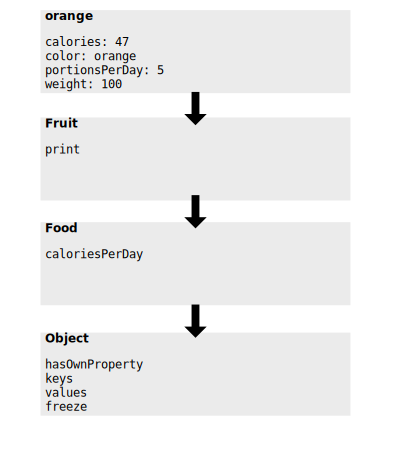
\includegraphics{/home/arran/projects/ExpoSE/Report/prototypechain}
\caption{}
\end{figure}

\hypertarget{header-n185}{%
\subsection{4.1.3 Arrays}\label{header-n185}}

Unlike other languages, JavaScript does not model arrays as continuously
indexed tuples. Instead arrays are a special form of object where array
elements are properties that satisfy the following test for a key
\texttt{k},
\texttt{ToString(ToUint32(k))\ ===\ k\ \&\&\ ToUint32(k)\ !==\ 2\^{}32\ -\ 1}.
In simpler terms, an array is a special case of an object where the
array elements are any value where the property can be coerced to a a
positive integer number less than 2\textsuperscript{32} - 1. These array
elements are treated differently to regular properties by array
prototypes and the length property.

The length of an array is a property of the array prototype which tracks
the highest index in the array. Note, that the highest index of the
array does not necessarily track the number of elements in the array as
arrays do not enforce any kind of ordering on their properties making it
possible to create a non-contiguous array, an array with 'holes' in it,
as shown in the example below. The length product is not read-only as
you might expect. If you increase length empty elements will be added to
the end of the array and decreasing the length will truncate the array
to satisfy the new length.

\begin{Shaded}
\begin{Highlighting}[]
\KeywordTok{let}\NormalTok{ arr }\OperatorTok{=}\NormalTok{ [] }\CommentTok{// an empty array}
\NormalTok{arr[}\DecValTok{0}\NormalTok{] }\OperatorTok{=} \DecValTok{0}
\NormalTok{arr[}\DecValTok{2}\NormalTok{] }\OperatorTok{=} \DecValTok{2}
\NormalTok{arr}
\OperatorTok{<}\NormalTok{ [}\DecValTok{0}\OperatorTok{,} \OperatorTok{,} \DecValTok{2}\NormalTok{]}
\VariableTok{arr}\NormalTok{.}\AttributeTok{length} 
\OperatorTok{<} \DecValTok{3}
\end{Highlighting}
\end{Shaded}

Another by-product of arrays being a special form of object is that
arrays are not homogenously typed. Whilst most languages require arrays
to only hold values of a single type, JavaScript objects and by
extension arrays can contain multiple types of value as shown by the
following example
\texttt{let\ array\ =\ {[}\textquotesingle{}a\textquotesingle{},\ 2.0,\ \{\},\ new\ Fruit(){]}}
.

As described above, arrays can have both properties and array elements.
If the property fails the array element test described above, then the
value is stored as a regular object value. This can lead to subtle bugs
when working with numbers if bounds are not checked as values smaller
than 0 and greater than 2\textsuperscript{32} - 1 will not be stored as
an array element, as demonstrated below.

\begin{Shaded}
\begin{Highlighting}[]
\KeywordTok{let}\NormalTok{ arr }\OperatorTok{=}\NormalTok{ []}
\NormalTok{arr[}\DecValTok{0}\NormalTok{] }\OperatorTok{=} \StringTok{'foo'} \CommentTok{// array element}
\VariableTok{arr}\NormalTok{.}\AttributeTok{length}
\OperatorTok{>} \DecValTok{1}
\NormalTok{arr[}\DecValTok{4294967296}\NormalTok{] }\OperatorTok{=} \StringTok{'bar'} \CommentTok{// 4294967296 === 2^32-1, property not an element}
\NormalTok{arr[}\OperatorTok{-}\DecValTok{1}\NormalTok{] }\OperatorTok{=} \StringTok{'baz'} \CommentTok{// -1 < 0, property not an element}
\VariableTok{arr}\NormalTok{.}\AttributeTok{length}
\OperatorTok{>} \DecValTok{1}
\NormalTok{arr[}\DecValTok{4294967296}\NormalTok{]}
\OperatorTok{>} \StringTok{'bar'}
\NormalTok{arr[}\OperatorTok{-}\DecValTok{1}\NormalTok{]}
\OperatorTok{>} \StringTok{'baz'}
\end{Highlighting}
\end{Shaded}

\hypertarget{header-n196}{%
\subsubsection{Prototype Methods}\label{header-n196}}

The array prototype has a large number of helper functions which
developers frequently take advantage of, a number of which were added in
the latest version of the EMCAScript standard \footnote{ECMA-262 6th
  Edition, The ECMAScript 2015 Language Specification. (2015). ECMA.}.
Below are some of the more commonly used and interesting functions.

\begin{longtable}[]{@{}lll@{}}
\toprule
Function Name & Signature & Description\tabularnewline
\midrule
\endhead
indexOf & \texttt{indexOf(element)} & Returns the first index of the
array that contains \texttt{element} or -1 if \texttt{element} is not in
the array\tabularnewline
lastIndexOf & \texttt{lastIndexOf(element)} & Returns the last index of
the array that contains \texttt{element} or -1 if element is not in the
array\tabularnewline
slice & \texttt{slice(begin,\ end)} & Returns a copy of the array with
the elements from the index \texttt{begin} up to the \texttt{end} index.
If \texttt{end} is not provided it will slice from \texttt{begin} to the
last element of the array\tabularnewline
push & \texttt{push(element)} & Increases the length of the array by one
and adds \texttt{element} to the end of the array\tabularnewline
pop & \texttt{pop()} & Removes the last element in the array and returns
it\tabularnewline
unShift & \texttt{unShift(elementA,\ elementB,\ ...)} & Adds one or more
elements to the beginning of an array and returns the new
length\tabularnewline
includes & \texttt{includes(element,\ startIndex)} & Returns true if the
array contains element either starting from \texttt{startIndex} or the
start of the array if no\texttt{startIndex} is provided\tabularnewline
reverse & \texttt{reverse()} & Reverses the array in place and returns a
reference to the array\tabularnewline
forEach & \texttt{forEach(func)} & Calls \texttt{func} on each element
in the array. Calls \texttt{func} with
\texttt{(value,\ index,\ array)}\tabularnewline
filter & \texttt{filter(func)} & Returns a new array that contains
elements that return true when \texttt{func} is called on them.
\texttt{func} is called with \texttt{currentElement}\tabularnewline
map & \texttt{map(func)} & Returns a new array with the results of
calling \texttt{func} on each element in the array. \texttt{func} is
called with \texttt{(value,\ index,\ array)}\tabularnewline
reduce & \texttt{reduce(func,\ initialValue)} & Calls
\texttt{func(accumulator,\ value,\ index,\ array)} on every element in
the array and returns the value of accumulator. If \texttt{initialValue}
is provided then the first time \texttt{func} is called then
\texttt{accumulator} is set to the value of
\texttt{initialValue}\tabularnewline
some & \texttt{some(func)} & Calls
\texttt{func(element,\ index,\ array)} for every element in the array.
Returns true if \texttt{func} returns true for at least one element in
the array\tabularnewline
every & \texttt{every(func)} & Calls
\texttt{func(element,\ index,\ array)} for every element in the array.
Returns true if \texttt{func} returns true for all elements in the
array\tabularnewline
\bottomrule
\end{longtable}

\hypertarget{header-n260}{%
\section{4.2 Ensuring the Correctness of JavaScript}\label{header-n260}}

As described in 1.1, assuring the correctness of JavaScript code is an
unsolved problem - in part due to the fact JavaScript is a dynamically
typed scripting language but also due to legacy design decisions.
Efforts have been made to make the language itself safer to use, for
example ECMAScript 5 introduced a strict mode (later made the default
mode in ECMAScript 6) which restricts the use of certain language
features and also defines additional circumstances that exceptions
should be thrown. However there are still many subtle errors that can
occur even within the safer subset of JavaScript.

Tools like Eslint and Flow are commonly used by developers to statically
analyse code and identify bugs but are limited in their scope. Eslint
uses a narrow set of rules to identify possibly dangerous behaviour and
Flow is constrained to reasoning about types and in some cases requires
additional code annotation to allow Flow to identify possible errors.
These limited sets of warnings do not fully reflect the dynamic nature
of JavaScript and the subtle interactions that can occur due to
prototypical inheritance, dynamic property access, and dynamic dispatch.
There have been a number of attempts to analyse JavaScript statically
however most approaches fall short of useful due to their inability to
reason about functions like \texttt{call()} and \texttt{apply()}
\footnote{Sridharan, M., Dolby, J., Chandra, S., Schäfer, M., \& Tip, F.
  (2012). Correlation tracking for points-to analysis of JavaScript.
  \emph{ECOOP 2012--Object-Oriented Programming}, 435-458.} with the
best results requiring an element of dynamic analysis as well.
\footnote{Logozzo, F., \& Venter, H. (2010). RATA: rapid atomic type
  analysis by abstract interpretation--application to javascript
  optimization. In \emph{Compiler Construction} (pp. 66-83). Springer
  Berlin/Heidelberg.} \footnote{Wei, S., \& Ryder, B. G. (2013, July).
  Practical blended taint analysis for JavaScript. In \emph{Proceedings
  of the 2013 International Symposium on Software Testing and Analysis}
  (pp. 336-346). ACM.}

Consequently there has been a shift in interest towards analysing safer
(and less dynamic) targets which compile to JavaScript, the most popular
of which is Typescript. Typescript is a superset of ECMAScript 6 which
includes optional types to enable errors to be caught statically before
compilation. Although TypeScript makes it easier to reason about
potential errors caused by coercion, TypeScript itself provides no
guarantees of static soundness - it's still possible for a TypeScript
program to compile to JavaScript successfully and encounter a run-time
error as a result of type coercion when executed. \footnote{Bierman, G.,
  Abadi, M., \& Torgersen, M. (2014, July). Understanding typescript. In
  \emph{European Conference on Object-Oriented Programming} (pp.
  257-281). Springer, Berlin, Heidelberg.} Extensions to TypeScript have
been suggested to provide soundness \footnote{Richards, G., Zappa
  Nardelli, F., \& Vitek, J. (2015). Concrete types for TypeScript. In
  \emph{LIPIcs-Leibniz International Proceedings in Informatics} (Vol.
  37). Schloss Dagstuhl-Leibniz-Zentrum fuer Informatik.} \footnote{Rastogi,
  A., Swamy, N., Fournet, C., Bierman, G., \& Vekris, P. (2015,
  January). Safe \& efficient gradual typing for TypeScript. In
  \emph{ACM SIGPLAN Notices} (Vol. 50, No. 1, pp. 167-180). ACM.}
although these approaches require a modified interpreter or runtime
enforcement. Regardless of , whilst TypeScript and its derivatives
provide a way of reducing or eliminating type based errors they don't
help identify or eliminate errors that occur due to other dynamic
features of JavaScript such as prototypical inheritance, dynamic
property access, or dynamic dispatch.

There most have been a number of attempts to produce formal semantics
for JavaScript, to allow for better reasoning about JavaScript code
however no attempts can be considered completely successful. One
approach taken by Philippa Gardner et al. (JaVerT) \footnote{Gardner, P.
  A., Maffeis, S., \& Smith, G. D. (2012). Towards a program logic for
  JavaScript. \emph{ACM SIGPLAN Notices}, \emph{47}(1), 31-44.}
\footnote{Guha, A., Saftoiu, C., \& Krishnamurthi, S. (2010, June). The
  essence of JavaScript. In \emph{European conference on Object-oriented
  programming} (pp. 126-150). Springer, Berlin, Heidelberg.} is to
translate a subset of the JavaScript language (targeting ECMAScript 5 in
strict mode) to an intermediate language, JSL, and then performing
analysis on JSL. Although the results of their analysis with translated
code is promising, their process and toolchain requires an expert level
understanding of the semantics of JavaScript and developers to annotate
their code pre and post-conditions. Although, this approach may be
suited for smaller programs (or critical subsets of programs) its
approach does not scale well to large applications. Other approaches
such a KJS \footnote{Park, D., Stefănescu, A., \& Roşu, G. (2015, June).
  KJS: A complete formal semantics of JavaScript. In \emph{ACM SIGPLAN
  Notices} (Vol. 50, No. 6, pp. 346-356). ACM.} and λJS \footnote{Guha,
  A., Saftoiu, C., \& Krishnamurthi, S. (2010, June). The essence of
  JavaScript. In \emph{European conference on Object-oriented
  programming} (pp. 126-150). Springer, Berlin, Heidelberg.} support
even less of the language than JaVerT and crucially none of the three
approaches target the ECMAScript 6 specification.

Symbolic execution provides an ideal way to test JavaScript code. By
concretely executing the program reasoning about the dynamic nature of
JavaScript is deferred this to the interpreter. The use of an
interpreter for testing also provides flexibility, if JavaScript needs
to be tested in another environment, switching interpreter is a
relatively easy change to make. Additionally, concrete execution comes
without the penalty of having to model the entire language specification
as any non-modelled function can simply revert to concrete execution.
Finally, symbolic execution is also able to test any JavaScript
underlying library code.

ExpoSE is a tool for symbolic execution of JavaScript. The target
program is instrumented with Jalangi2, a tool that provides hooks before
and after each statement is executed, which is used to build a symbolic
representation of the program. ExpoSE uses a harness to randomly
generate inputs for public functions in a target JavaScript program. It
then uses a DART\footnote{Godefroid, P., Klarlund, N., \& Sen, K. (2005,
  June). DART: directed automated random testing. In \emph{ACM Sigplan
  Notices} (Vol. 40, No. 6, pp. 213-223). ACM.} based directed search to
attempt to explore all feasible paths in the program up to a maximum
path count. Constraints are solved using Z3, a Microsoft Research
theorem prover.

\hypertarget{header-n273}{%
\section{5 SMT}\label{header-n273}}

\hypertarget{header-n274}{%
\section{6 Results}\label{header-n274}}

\hypertarget{header-n275}{%
\section{7 Conclusion}\label{header-n275}}

\hypertarget{header-n276}{%
\section{Bibliography}\label{header-n276}}

\end{document}
